\documentclass[11pt]{article}

% Setting up the page
\usepackage{setspace}
    \newcommand{\standardspacing}{\singlespacing}
    \standardspacing%
\usepackage[english]{babel}
\usepackage[utf8]{inputenc}
\usepackage{fullpage}

% Bibliography
\usepackage[numbers]{natbib}
\bibliographystyle{abbrvnat}

% Writing mathematics, algorithms and code
\usepackage{mathtools}
\usepackage{multicol}
\usepackage{enumitem}
\usepackage{amsmath}
\usepackage{amssymb}
\usepackage[boxruled]{algorithm2e}

\newcommand{\balg}{\begin{algorithm}[htbp]\DontPrintSemicolon\singlespacing}
\newcommand{\ealg}{\end{algorithm}\standardspacing}

\DeclarePairedDelimiter\abs{\lvert}{\rvert}%
\DeclarePairedDelimiter\norm{\lVert}{\rVert}%

% Images, tables and referencing
\usepackage{graphicx}
    \newcommand{\imgwidth}{.85\textwidth}
\usepackage{tikz}
\usepackage{xcolor}
\usepackage{hyperref}
\usepackage{caption}
\usepackage{booktabs}
\usepackage{float}

% For indexing sections, etc.
\usepackage{amsthm}
\theoremstyle{definition} \newtheorem{definition}{Definition}[section]
\newtheorem*{remark}{Remark}
\newtheorem{theorem}{Theorem}

\title{%
    A novel game-theoretic initialisation process for the \(k\)-modes
    algorithm using the hospital-resident assignment problem
}
\author{Henry Wilde, Vincent Knight and Jonathan Gillard}

\begin{document}

\maketitle%
\begin{abstract}\singlespacing%
    The \(k\)-modes algorithm is a centroid-based clustering algorithm, and is
    an extension of the \(k\)-means algorithm for categorical data. This work
    outlines a comparison of the established initialisation methods
    for the \(k\)-modes algorithm by use of examples and algebraic analysis of
    their cost functions. In doing so, the effect of the initial centroid
    selection on the overall efficiency and quality of the final clustering
    found by each method is exposed.

    Following this, a novel initialisation process is described that utilises
    game-theoretic results to create a fair and robust initial selection for the
    algorithm. This process is modelled on the hospital-resident assignment
    problem and is solved using an adapted Gale-Shapley algorithm.

    The paper concludes with a comparison between the established initialisation
    methods and the proposed method on a number of benchmark datasets, as well
    as an analysis using preferable artificial datasets. The analysis uses
    several label-invariant metrics to assess the quality of the clustering both
    at the beginning of the algorithm and at the end.
\end{abstract}\doublespacing%

\section{Introduction}\label{sec:intro}

\begin{itemize}
    \item What is clustering?
    \item What is the \(k\)-means paradigm?
    \item What is categorical data and how is it clustered?
\end{itemize}

\subsection{The \(k\)-modes algorithm}\label{subsec:kmodes}

The following notation will be used throughout this work to describe the objects
associated with clustering a dataset:

\begin{itemize}
    \item Let \(\mathcal{A} := A_1 \times \cdots \times A_m\) denote the
        \emph{attribute~space}. In this work, only categorical attributes are
        considered and so it is intuitive to describe each attribute as a set of
        its values, i.e.\ for each \(j = 1, \ldots, m\) it follows that \(A_j :=
        \left\{a_1^{(j)}, \ldots, a_{d_j}^{(j)}\right\}\) where \(d_j = |A_j|\)
        is considered the size of the \(j^{th}\) attribute.

    \item Let \(\mathcal{X} := \left\{X^{(1)}, \ldots, X^{(N)}\right\} \subset
        \mathcal{A}\) denote a \emph{dataset} where each \(X^{(i)} \in
        \mathcal{X}\) is defined as an \(m\)-tuple \(X^{(i)} := \left(x_1^{(i)},
        \ldots, x_m^{(i)}\right)\) where \(x_j^{(i)} \in A_j\) for each \(j = 1,
        \ldots, m\). The elements of \(\mathcal{X}\) are referred to as
        \emph{data points} or \emph{instances}.
%        A dataset \(\mathcal{X}\) can be
%        represented as a table like so:
%        \begin{table}[H]
%        \centering
%        \begin{tabular}{cccccc}
%            {} & \(A_1\) & \(A_2\) & \quad \ldots \quad & \(A_{m-1}\) & \(A_m\)
%            \\
%            \midrule
%            \(X^{(1)}\) & \(x_1^{(1)}\) & \(x_2^{(1)}\) & \quad \ldots \quad & 
%            \(x_{m-1}^{(1)}\) & \(x_m^{(1)}\)
%            \\
%            \(X^{(2)}\) & \(x_1^{(2)}\) & \(x_2^{(2)}\) & \quad \ldots \quad &
%            \(x_{m-1}^{(2)}\) & \(x_m^{(2)}\)
%            \\
%            \vdots & \vdots & \vdots & {} & \vdots & \vdots
%            \\
%            \(X^{(N)}\) & \(x_1^{(N)}\) & \(x_2^{(N)}\) & \quad \ldots \quad &
%            \(x_{m-1}^{(N)}\) & \(x_m^{(N)}\)
%        \end{tabular}
%        \end{table}

    \item Let \(\mathcal{Z} := \left(Z_1, \ldots, Z_k\right)\) be a partition
        of a dataset \(\mathcal{X}\) into \(k \in \mathbb{Z}^{+}\) distinct,
        non-empty parts. Such a partition \(\mathcal{Z}\) is called a
        \emph{clustering} of \(\mathcal{X}\).

    \item Each cluster \(Z_l\) has associated with it a
        \emph{representative~point} (see Definition~\ref{def:mode}) which is
        denoted by \(z^{(l)} = \left(z_1^{(l)},~\ldots,~z_m^{(l)}\right) \in
        \mathcal{A}\).  These points may also be referred to as cluster modes.
        The set of all current representative points is denoted \(\overline Z =
        \left\{z^{(1)}, \ldots, z^{(k)}\right\}\).
\end{itemize}

As is discussed above, the notion of distance is lost in categorical space, and
especially when that space is even partly nominal. Definition~\ref{def:dissim}
describes a simple dissimilarity measure between categorical data points.

\begin{definition}\label{def:dissim}
    Let \(\mathcal{X}\) be a dataset and consider any \(X^{(a)}, X^{(b)} \in
    \mathcal{X}\). The dissimilarity between \(X^{(a)}\) and \(X^{(b)}\),
    denoted by \(d\left(X^{(a)}, X^{(b)}\right)\), is given by:
    \begin{equation}\label{eq:dissim}
        d\left(X^{(a)}, X^{(b)}\right) := \sum_{j=1}^{m} \delta\left(x_j^{(a)},
        x_j^{(b)}\right) \quad \text{where} \quad \delta\left(x, y\right) =
        \begin{cases}
            0, & \text{if} \ x = y \\
            1, & \text{otherwise.}
        \end{cases}
    \end{equation}
    In other words, the dissimilarity between two points is the number of
    attributes where their values are not the same. A proof
    that~\eqref{eq:dissim} is a valid distance metric is given as an appendix.
\end{definition}

%\begin{example}\label{ex:dissim}
    Throughout this work, we will make use of a number of small examples to aid
    our understanding of various concepts. These examples will utilise a small,
    artificial dataset describing some qualities about vehicles.
    
    The dataset is made up of \(N = 10\) instances, each of which describe a
    vehicle. These instances are defined by \(m = 6\) attributes, the first two
    of which are ordinal variables taken from the set \(\{\text{L, M, H, V}\}\)
    standing for `low', `medium', `high', and `very high' respectively. The
    next three are integer variables and so can be considered as categorical,
    and the final attribute is a binary variable indicating whether the vehicle
    is eco-friendly \((1)\) or not \((0)\). The full dataset is given in
    Table~\ref{tab:dataset}. Please note that there is an additional, unheaded
    column on the left hand side showing the index starting at \(1\) and going
    up to \(5\).
    
    \begin{table}[H]
        \centering
        \singlespacing{%
        \resizebox{.8\textwidth}{!}{%
            \centering
            \begin{tabular}{ccccccc}
\toprule
{} & Buying price & Maintenance costs & No. doors & No. passengers & No. wheels & Eco-friendly \\
\midrule
1  &            H &                 M &         2 &              2 &          4 &            0 \\
2  &            L &                 M &         0 &              1 &          2 &            0 \\
3  &            V &                 H &         2 &              3 &          8 &            0 \\
4  &            H &                 L &         4 &              5 &          4 &            1 \\
5  &            M &                 M &         2 &              5 &          4 &            1 \\
6  &            M &                 L &         2 &              4 &          4 &            1 \\
7  &            V &                 H &         4 &              5 &          4 &            0 \\
8  &            L &                 V &         2 &              4 &          4 &            0 \\
9  &            H &                 M &         0 &              2 &          2 &            1 \\
10 &            H &                 M &         4 &              7 &          4 &            0 \\
\bottomrule
\end{tabular}

        }}
        \caption{The vehicle dataset.}\label{tab:dataset}
    \end{table}

    Let us consider our first two datapoints. With the notation laid out in
    Section~\ref{subsec:notation}, we can express these points as vectors in the
    following way:

    \begin{equation}
        \nonumber
        \begin{aligned}
            X^{(1)} & = & \left[ x_1^{(1)} = \text{H}, \ x_2^{(1)} = \text{M}, \
            x_3^{(1)} = 2, \ x_4^{(1)} = 2, \ x_5^{(1)} = 4, \ x_6^{(1)} = 0 
            \right]
            \\
            X^{(2)} & = & \left[ x_1^{(2)} = \text{L}, \ x_2^{(2)} = \text{M}, \
            x_3^{(2)} = 0, \ x_4^{(2)} = 1, \ x_5^{(2)} = 2, \ x_6^{(2)} = 0
            \right]
        \end{aligned}
    \end{equation}

    Then, by Definition~\ref{def:dissim}, their pairwise dissimilarity is:
    \begin{equation}
        \nonumber
        \begin{aligned}
            \centering
            d(X^{(1)}, X^{(2)}) & = & \delta(\text{H}, \text{L}) & + & 
            \delta(\text{M}, \text{M}) & + & \delta(3, 0) & + & \delta(2, 1) &
            + & \delta(4, 2) & + & \delta(0, 0) & {} & {}
            \\
            {} & = & 1 \ & + & 0 \ & + & 1 \ & + & 1 \ & + & 1 \ & + & 0 \ & = &
            4
        \end{aligned}
    \end{equation}
\end{example}


With this metric defined, the notion of a representative point within a cluster
can be addressed. When clustering numeric data, a centroid of a cluster is taken
to be the average of the points within the cluster so as to summarise the
information contained within that cluster. With categorical data, however, a
frequency approach is used. This follows from the concept of dissimilarity
where the point that best represents (i.e.\ is closest to) those in a cluster
is one with the most frequent attribute values of the points in the cluster. As
such, a representative point of a cluster is often called a mode. The following
definitions and theorem formally define such a representative point and a means
of finding them.

\begin{definition}\label{def:mode}
    Let \(\mathcal{X} \subset \mathcal{A}\) be a dataset and consider some point
    \(z = \left(z_1, \ldots, z_m\right) \in \mathcal{A}\). Then \(z\) is called
    a \emph{mode} of \(\mathcal{X}\) if it minimises the following:
    \begin{equation}\label{eq:summed-dissim}
        D\left(\mathcal{X}, z\right) = \sum_{i=1}^{N} d\left(X^{(i)}, z\right)
    \end{equation}
\end{definition}

\begin{definition}\label{def:rel-freq}
    Let \(\mathcal{X} \subset \mathcal{A}\) be a dataset. Then
    \(n\left(a_s^{(j)}\right)\) denotes the \emph{frequency} of the \(s^{th}\)
    category \(a_s^{(j)}\) of \(A_j\) in \(\mathcal{X}\), i.e.\ for each \(A_j
    \in \mathcal{A}\) and each \(s = 1, \ldots, d_j\):
    \begin{equation}
        n\left(a_s^{(j)}\right) := \abs*{%
            {\left\{X^{(i)} \in \mathcal{X}: x_j^{(i)} = a_s^{(j)}\right\}}
        }
    \end{equation}
	
    Furthermore, \(\frac{n\left(a_s^{(j)}\right)}{N}\) is called the
    \emph{relative~frequency} of category \(a_s^{(j)}\) in \(\mathcal{X}\).
\end{definition}

\begin{theorem}\label{thm:mode}
    Consider a dataset \(\mathcal{X} \subset \mathcal{A}\) and some \(U = (u_1,
    \ldots, u_m) \in \mathcal{A}\). Then \(D(\mathcal{X}, U)\) is minimised if
    and only if \(n\left(u_j\right) \geq n\left(a_s^{(j)}\right)\) for all
    \(s=1, \ldots, d_j\) for each \(j = 1, \ldots, m\).

    A proof of this theorem can be found in the Appendix of~\cite{Huang1998}.
\end{theorem}

%\begin{example}\label{ex:mode}
    Let us return to our vehicale dataset from Example~\ref{ex:dissim}. Using 
    Theorem~\ref{thm:1}, we can identify a mode of our set by taking the most 
    commonly occurring value for each attribute. We can then take these values
    as a vector and call it \(\mu\). In this case, we have:

    \[ 
 	 \mu = \left[\text{H}, \ \text{M}, \ \text{2}, \ \text{5}, \ \text{4}, \ \text{0}\right] 
\]

    This point actually appears in our dataset and corresponds to the first row.
    It is easily verified (a Python script doing so is given as an Appendix)
    that this point is in fact the only point in the span of the attribute space
    \(A_1 \times \cdots \times A_6\) that minimises our summed dissimilarity. In
    this way, we have that the first row of our dataset is the only true mode of
    our set, virtual or not.
\end{example}



Theorem~\ref{thm:mode} defines the process by which representatives are updated
in \(k\)-modes (see Algorithm~\ref{alg:update}), and so the final component from
the \(k\)-means paradigm to be configured is the objective (cost) function. This
function is defined in Definition~\ref{def:cost}, and following that a practical
statement of the \(k\)-modes algorithm is given in Algorithm~\ref{alg:kmodes} as
set out in~\cite{Huang1998}.

\begin{definition}\label{def:cost}
    Let \(\mathcal{Z} = \left\{Z_1, \ldots, Z_k\right\}\) be a clustering of a
    dataset \(\mathcal{X}\), and let \(\overline Z = \left\{z^{(1)},
    \ldots, z^{(k)}\right\}\) be the corresponding cluster modes. Then \(W =
    \left(w_{i, l}\right)\) is an \(N \times k\) \emph{partition~matrix} of
    \(\mathcal{X}\) such that:
    \[
        w_{i, l} = \begin{cases}
                     1, & \text{if} \ X^{(i)} \in Z_l\\
                     0, & \text{otherwise.}
                   \end{cases}
    \]

    With this, the \emph{cost~function} is defined to be the summed
    within-cluster dissimilarity:
    \begin{equation}
        C\left(W, \overline Z\right) := \sum_{l=1}^{k} \sum_{i=1}^{N}
        \sum_{j=1}^{m} w_{i,l} \ \delta\left(x_j^{(i)}, z_j^{(l)}\right)
    \end{equation}
\end{definition}

\balg%
    \caption{The \(k\)-modes algorithm}\label{alg:kmodes}
    \KwIn{a dataset \(\mathcal{X}\), a number of clusters to form \(k\)}
    \KwOut{a clustering \(\mathcal{Z}\) of \(\mathcal{X}\)}

    Select \(k\) initial modes \(z^{(1)}, \ldots, z^{(k)} \in \mathcal{X}\)\;
    \(\overline Z \gets \left\{z^{(1)}, \ldots, z^{(k)}\right\}\)\;
    \(\mathcal{Z} \gets \left(\left\{z^{(1)}\right\}, \ldots,
    \left\{z^{(k)}\right\}\right)\)\;

    \For{\(X^{(i)} \in \mathcal{X}\)}{%
        \(Z_{l^*} \gets \textsc{SelectClosest}\left(X^{(i)}\right)\)\;
        \(Z_{l^*} \gets Z_{l^*} \cup \left\{X^{(i)}\right\}\)\;
        \(\textsc{Update}\left(z^{(l^*)}\right)\)\;
    }

    \Repeat{No point changes cluster}{%
        \For{\(X^{(i)} \in \textbf{X}\)}{%
            Let \(Z_l\) be the cluster \(X^{(i)}\) currently belongs to\;
            \(Z_{l^*} \gets \textsc{SelectClosest}\left(X^{(i)}\right)\)\;
            \If{\(l \neq l^*\)}{%                
                \(Z_{l} \gets Z_{l} \setminus \left\{X^{(i)}\right\}\) and
                \(Z_{l^*} \gets Z_{l^*} \cup \left\{X^{(i)}\right\}\)\;
                \(\textsc{Update}\left(z^{(l)}\right)\) and
                \(\textsc{Update}\left(z^{(l^*)}\right)\)\;
            }
        }
    }
\ealg%

\balg%
    \caption{\textsc{SelectClosest}}\label{alg:select_closest}
    \KwIn{%
        a data point \(X^{(i)}\), a set of current clusters \(mathcal{Z}\) and
        their modes \(\overline Z\)
    }
    \KwOut{the cluster whose mode is closest to the data point \(Z_{l^*}\)}

    Select \(z^{l^*} \in \overline Z\) that minimises:
    \(d\left(X^{(i)}, z_{l^*}\right)\)\;
    Find their associated cluster \(Z_{l^*}\)
\ealg%

\balg%
    \caption{\textsc{Update}}
    \KwIn{an attribute space \(\mathcal{A}\), a mode to update \(z^{(l)}\) and
    its cluster \(Z_l\)}
    \KwOut{an updated mode}

    Find \(z \in \mathcal{A}\) that minimises \(D(Z_l, z)\)\;
    \(z^{(l)} \gets z\)\;
\ealg%



\subsection{Initialisation processes}\label{subsec:inits}

The \(k\)-modes algorithm is a heuristic so its performance is dependent on the
its initial solution. The quality of the initial centroids for a particular
dataset is affected by two components: the metric attached to the attribute
space and the process by which they are chosen.

Following the seminal \(k\)-modes papers~\cite{Huang1997a,Huang1997b,Huang1998},
a number of alternative dissimilarity measures have been implemented to improve
on the simple matching dissimilarity defined in~\eqref{eq:dissim}. The main
drawback of this measure is that it often produces clusters with low
intra-cluster similarity~\cite{Ng2007} and does not take into account any
relationships between attributes or their categories. Other measures have been
designed to be used in a specific context where such relationships may be
considered~\cite{Cao2012,Yu2018,Zhou2016}.

This work considers, instead, the process by which the initial modes are
selected. The standard selection method is to randomly sample \(k\) distinct
points in the dataset. In all cases, the initial modes must be points in the
dataset to ensure that there are no empty clusters in the first iteration of the
algorithm. The remainder of this section describes two well-established
initialisation methods that aim to preemptively lever the structure of the data
at hand.

\subsubsection{Huang's method}\label{subsec:huang}

Amongst the original works by Huang, an alternative initialisation method was
presented that selects modes by forcing diversity amongst them~\cite{Huang1998}.
The process, denoted as Huang's method, is described in full in
Algorithm~\ref{alg:huang}. Huang's method considers a set of potential modes,
\(\widehat Z \subset \mathcal A\), that is then replaced by the actual set of
initial modes, \(\overline Z \subset \mathcal X\).

In the original statement of Huang's method, it is stated that the most
frequent categories should be assigned `equally' to the set of potential modes.
How the categories should be distributed `equally' is not well-defined or easily
seen from the example given in the paper. In software implementations, including
the one used in Section~\ref{sec:results}, the term is taken to mean using a
probability distribution to sample values from the attribute space. This
probability distribution is formed by the relative frequencies of each
attribute's categories.

\begin{algorithm}[H]
\caption{Huang's method}\label{alg:huang}
    \begin{algorithmic}[0]
        \State{\textbf{Input:} a dataset \textbf{X}, with attribute sets \(A_1,
        \ldots, A_m\), and a number of modes to find \(k\)}
        \State{\textbf{Output:} a set of \(k\) initial modes \(\bar{\mu}\)\\}
        \\
        \Comment{Initialisation step}
        \State{\(\tilde{\mu} \gets \emptyset\)}
        \State{\(\bar{\mu} \gets \emptyset\)}
        \For{\(j = 1, \ldots, m\)}
            \For{\(s = 1, \ldots, d_j\)}
                \State{Calculate the relative frequency of each attribute value:
                    \(\frac{n(a_s^{(j)})}{N}\).}
	        \EndFor
        \EndFor
        \\
        \\
        \Comment{Distribute most common attribute values}
        \For{\(l = 1, \ldots, k\)}
            \For{\(j = 1, \ldots, m\)}
                \State{Sample \(a_{s^*}^{(j)}\) from \(A_j\) by considering the 
                relative frequencies of the elements of \(A_j\) as a probability
                distribution.}
                \State{\(\mu_j^{(l)} \gets a_{s^*}^{(j)}\)}
	        \EndFor
            \State{\(\tilde{\mu} \gets \tilde{\mu} \cup \{\mu^{(l)}\}\)}
	    \EndFor
        \\
        \\
        \Comment{Replace \(\tilde{\mu}\) with points in \textbf{X} to avoid
        empty clusters}
        \For{\(\mu \in \tilde{\mu}\)}
            \State{Select \(X^{(i^*)} \in \textbf{X}\) such that: 
                \[
                    X^{(i^*)} = \argmin_{1 \leq i \leq N} \left\{ d(X^{(i)}, 
                    \mu): \ X^{(i^*)} \neq \mu'  \ \forall \mu' \in 
                    \bar{\mu}\right\}
                \]
            }
            \State{\(\bar{\mu} \gets \bar{\mu} \cup \left\{X^{(i^*)}\right\}\)}
        \EndFor
    \end{algorithmic}
\end{algorithm}

%\begin{example}\label{ex:huang}
    Consider our vehicle dataset. We will now find a set of initial modes for
    the \(k\)-modes algorithm using Huang's method. For the sake of this
    example, we will let \(k = 3\).
    
    \begin{table}[H]
    \centering
    \singlespacing{%
    \resizebox{.8\textwidth}{!}{%
        \begin{tabular}{lrrrrrr}
\toprule
{} &  Doors &  Eco-Friendly &  Maintenance &  Passengers &  Price &  Wheels \\
\midrule
0 &    0.2 &           0.6 &          0.0 &         0.0 &    0.0 &     0.0 \\
1 &    0.0 &           0.4 &          0.0 &         0.1 &    0.0 &     0.0 \\
2 &    0.5 &           0.0 &          0.0 &         0.2 &    0.0 &     0.2 \\
3 &    0.0 &           0.0 &          0.0 &         0.1 &    0.0 &     0.0 \\
4 &    0.3 &           0.0 &          0.0 &         0.2 &    0.0 &     0.7 \\
5 &    0.0 &           0.0 &          0.0 &         0.3 &    0.0 &     0.0 \\
7 &    0.0 &           0.0 &          0.0 &         0.1 &    0.0 &     0.0 \\
8 &    0.0 &           0.0 &          0.0 &         0.0 &    0.0 &     0.1 \\
L &    0.0 &           0.0 &          0.2 &         0.0 &    0.2 &     0.0 \\
M &    0.0 &           0.0 &          0.5 &         0.0 &    0.2 &     0.0 \\
H &    0.0 &           0.0 &          0.2 &         0.0 &    0.4 &     0.0 \\
V &    0.0 &           0.0 &          0.1 &         0.0 &    0.2 &     0.0 \\
\bottomrule
\end{tabular}

    }}
    \caption{Relative frequency table for attribute values.}\label{tab:rel-freq}
    \end{table}

    We begin by calculating the relative frequencies of our attributes' values,
    which are stored in Table~\ref{tab:rel-freq}. Now to find our set of
    (potentially) virtual modes, \(\tilde{\mu}\). For each attribute, we will
    take a sample of size one from the its set of values according to the
    probability distribution represented in the corresponding column of
    Table~\ref{tab:rel-freq}. Let us begin with the first attribute of our first
    mode in \(\tilde{\mu}\). Then we have to sample from the following
    probability distribution:
    
    \begin{table}[H]
    \centering
    \singlespacing{%
    \begin{tabular}{cccccc}
        \(A_{1}\) &\vline& L & M & H & V \\
        \midrule\(\mathbb{P}(A_{1} = a_s^{(1)})\) &\vline& \(\frac{2}{10}\) &
        \(\frac{2}{10}\) & \(\frac{4}{10}\) & \(\frac{2}{10}\) 
    \end{tabular}
    }
    \end{table}
    
    We sample one value from this distribution and set that value to be the
    first component of our first mode. This process is repeated for all values
    \(l = 1, 2, 3\) and \(j = 1, \ldots, 6\) giving us \(3\) \(m\)-dimensional
    vectors that fairly represent the most frequent attribute values. This set
    of vectors is \(\tilde{\mu}\).

    There are many ways of obtaining \(\tilde{\mu}\) from our relative frequency
    table but we have opted to do so using a short Python script (see Appendix).
    In this case, we have the following set of vectors:

    \begin{equation} 
\begin{aligned} 
	\tilde{\mu} = \left\{ & \left[\text{L}, \ \text{M}, \ \text{4}, \ \text{2}, \ \text{4}, \ \text{0}\right], \\ & \left[\text{H}, \ \text{M}, \ \text{0}, \ \text{4}, \ \text{2}, \ \text{1}\right], \\ & \left[\text{H}, \ \text{M}, \ \text{2}, \ \text{4}, \ \text{4}, \ \text{0}\right]\right\} \\ 
\end{aligned} 
\end{equation}

    Finally, we take each element of \(\tilde{\mu}\) in turn and find its most
    similar point in the dataset. This collection of points in the dataset then
    forms our set of initial modes \(\bar{\mu}\) to be passed on to the 
    \(k\)-modes algorithm. We stipulate that no point which is identical to
    another that has been already selected may be used as an initial mode. This
    is done so as to avoid empty clusters further down the line.

    \begin{table}[H]
    \centering
    \singlespacing{%
    \resizebox{.8\textwidth}{!}{%
        \begin{tabular}{lllllllr}
\toprule
{} & Price & Maintenance & Doors & Passengers & Wheels & Eco-Friendly &  Dissimilarity to \$\textbackslashtilde\{\textbackslashmu\}\_1\$ \\
\midrule
5 &     M &           L &     2 &          4 &      4 &            1 &                                 1 \\
7 &     L &           V &     2 &          4 &      4 &            0 &                                 2 \\
3 &     H &           L &     4 &          5 &      4 &            1 &                                 3 \\
4 &     M &           M &     2 &          5 &      4 &            1 &                                 3 \\
0 &     H &           M &     2 &          2 &      4 &            0 &                                 4 \\
1 &     L &           M &     0 &          1 &      2 &            0 &                                 5 \\
2 &     V &           H &     2 &          3 &      8 &            0 &                                 5 \\
6 &     V &           H &     4 &          5 &      4 &            0 &                                 5 \\
8 &     H &           M &     0 &          2 &      2 &            1 &                                 5 \\
9 &     H &           M &     4 &          7 &      4 &            0 &                                 5 \\
\bottomrule
\end{tabular}

    }}
    \caption{The dataset ranked by dissimilarity to the first element of
    \(\tilde{\mu}\).}\label{tab:huang-mode-dissim}
    \end{table}

    Taking the first element of \(\tilde{\mu}\), we calculate the dissimilarity
    between this vector and all of our datapoints.
    Table~\ref{tab:huang-mode-dissim} shows the elements of our dataset ranked
    in ascending order of their dissimilarity to this vector. It follows that we
    should set our first initial mode to be the sixth entry of our dataset. We
    continue this process for the other elements of \(\tilde{\mu}\),
    disregarding any points that have already been selected.
    
    Using our Python implementation for Huang's initialisation method we have 
    that the set of initial modes for this instance of the \(k\)-modes algorithm
    correspond to the sixth, fifth and fourth rows of the dataset. That is, we
    have:

    \begin{equation}
\nonumber
\begin{aligned}
\bar{\mu} = \{  & \left[\text{2}, \ \text{1}, \ \text{L}, \ \text{4}, \ \text{M}, \ \text{4}\right], \\  & \left[\text{2}, \ \text{1}, \ \text{M}, \ \text{5}, \ \text{M}, \ \text{4}\right], \\  & \left[\text{4}, \ \text{1}, \ \text{L}, \ \text{5}, \ \text{H}, \ \text{4}\right]\} \\ 
\end{aligned}
\end{equation}
\end{example}




\subsubsection{Cao's method}\label{subsec:cao}

Cao's method selects representative points by the average density of a point in
the dataset. As will be seen in the following definition, this average density 
is in fact the average relative frequency of all the attribute values of that 
point. This method is considered deterministic as there is no probabilistic
element \- unlike Huang's method or a random initialisation. So, we can consider
the results to be largely reproducible, except in the case where a tie must be
broken (see Example~\ref{ex:cao}).

\begin{definition}\label{def:density}	
    Consider a data set \(\mathcal{X}\) with attribute set \(\mathcal{A} = 
    \{A_1, \ldots, A_m\}\). Then the \emph{average~density} of any point 
    \(X_i \in \mathcal{X}\) with respect to \(\mathcal{A}\) is 
    defined~\cite{Cao2009} as:
    \begin{equation}\label{eq:density}
        \text{Dens}\left(X^{(i)}\right) = \frac{%
            \sum_{j=1}^m \text{Dens}_{j}\left(X^{(i)}\right)
        }{m}
        \ \ \text{where} \ \
        \text{Dens}_{j}\left(X^{(i)}\right) = \frac{%
            \abs*{%
                \left\{X^{(t)} \in \mathcal{X} : x_j^{(i)} = x_j^{(t)}\right\}
            }
        }{N}
    \end{equation}

    Observe that:
    \[
        \abs*{\left\{X^{(t)} \in \mathcal{X} : x_j^{(i)} = x_j^{(t)}\right\}}%
        = n\left(x_j^{(i)}\right)%
        = \sum_{t=1}^N \left(1 - \delta\left(x_j^{(i)}, x_j^{(t)}\right)\right)
    \]

    And so, an alternative definition for~(\ref{eq:density}) can be derived:
    \begin{equation}\label{eq:density-alt}
    \begin{aligned}
        \text{Dens}\left(X^{(i)}\right)
        & = \frac{1}{mN} \sum_{j=1}^m \sum_{t=1}^N \left(%
            1 - \delta\left(x_j^{(i)}, x_j^{(t)}\right)
        \right)\\
        & = \frac{1}{mN} \sum_{j=1}^m \sum_{t=1}^N 1%
            - \frac{1}{mN} \sum_{j=1}^m \sum_{t=1}^N
            \delta\left(x_j^{(i)}, x_j^{(t)}\right)\\
        & = \frac{mN}{mN} - \frac{1}{mN} \sum_{t=1}^N
            d\left(X^{(i)}, X^{(t)}\right)\\
        & = 1 - \frac{1}{mN} D\left(\mathcal{X}, X^{(i)}\right)
    \end{aligned}
    \end{equation}
\end{definition}

\begin{remark}
    It is worth noting that for all \(X^{(i)} \in \mathcal{X}\) it follows that
    \(\frac{1}{N} \leq \text{Dens}\left(X^{(i)}\right)
    \leq 1\), since:		
	\begin{itemize}	
        \item If \(n\left(x_j^{(i)}\right) = 1\) for all \(j = 1, \ldots, m\)
            then \(%
                \text{Dens}\left(X^{(i)}\right)
                = \frac{\sum_{j=1}^m \frac{1}{N}}{m}
                = \frac{m}{mN}
                = \frac{1}{N}
            \).
        \item If \(n\left(x_j^{(i)}\right) = N\) for all \(j = 1, \ldots, m\)
            then \(%
                \text{Dens}\left(X^{(i)}\right)
                = \frac{\sum_{j=1}^m 1}{m}
                = \frac{m}{m}
                = 1
            \).
	\end{itemize}
\end{remark}

\begin{algorithm}[H]
\caption{Cao's method}\label{alg:cao}
	\begin{algorithmic}[0]
        \State{\textbf{Input:} a dataset \textbf{X}, with attribute sets \(A_1,
        \ldots, A_m\), and a number of modes to find \(k\)}
        \State{\textbf{Output:} a set of \(k\) initial modes \(\bar{\mu}\)\\}
        \\
        \Comment{Initialisation step}
        \State{\(\bar{\mu} \gets \emptyset\)}
        \For{\(X^{(i)} \in \textbf{X}\)}
            \State{Calculate \(\text{Dens}(X^{(i)})\).}
		\EndFor
        \\
        \\
        \Comment{Select the point with maximal density}
        \State{Select \(X^{(i_1)} \in \textbf{X}\) which satisfies:
        \[
            X^{(i_1)} = \argmax_{1 \leq i \leq N} 
            \left\{\text{Dens}(X^{(i)})\right\}
        \]
        }
        \State{\(\bar{\mu} \gets \bar{\mu} \cup X^{(i_1)}\)\\}
        \\
        \Comment{Second point maximises both density and distance from the first
        mode}
        \State{Select \(X^{(i_2)} \in \textbf{X}\) which satisfies: 
		\[
            X^{(i_2)} = \argmax_{1 \leq i \leq N} \left\{\text{Dens}(X^{(i)})
            \times d(X^{(i)}, X^{(i_1)})\right\}
		\]
        }
        \\
        \State{\(\bar{\mu} \gets \bar{\mu} \cup X^{(i_2)}\)\\}
        \\
        \Comment{Continue to choose points in this fashion until \(k\) are
        chosen}
        \While{\(|\bar{\mu}| < k\)}
            \State{Select \(X^{(i_3)} \in \textbf{X}\) which satisfies:
			\[
                X^{(i_3)} = \argmax_{1 \leq i \leq N} \left\{\min_{\mu^{(l)} \in
                \bar{\mu}} \left\{\text{Dens}(X^{(i)}) \times d(X^{i}, 
                \mu^{(l)})\right\}\right\}
			\]
            }
            \State{\(\bar{\mu} \gets \bar{\mu} \cup X^{(i_3)}\)}
		\EndWhile
	\end{algorithmic}
\end{algorithm}



\begin{remark}
    With this alternative definition, we see \-- since \(m\) and \(N\) are fixed
    positive integers \-- that \(\text{Dens}(X^{(i)})\) is maximised when
    \(D(\mathcal{X}, X^{(i)})\) is minimised. Then by Theorem~\ref{thm:1} we have
    that such an \(X^{(i)}\) with maximal average density in \(\mathcal{X}\)
    with respect to \(\mathcal{A}\) is, in fact, a mode of \(\mathcal{X}\). This
    observation allows us to consider some sense of similarity between Huang and
    Cao's methods, as they seem to be trying to achieve the same objective \--
    if only from opposite ends.
\end{remark}

%\begin{example}\label{ex:cao}
    We will now attempt to find \(3\) initial modes for our vehicle dataset 
    using Cao's method, as we did in Example~\ref{ex:huang}. We begin by 
    calculating the average density of each of our points. We rank these in 
    descending order, and take the point with maximal density as our first 
    initial mode. This ranking is shown in Table~\ref{tab:ranked-density}.

    \begin{table}[H]
        \centering
        \singlespacing{%
        \resizebox{.8\textwidth}{!}{%
            \begin{tabular}{cccccccc}
\toprule
{} & Buying price & Maintenance costs &  No. doors &  No. passengers &  No. wheels &  Eco-friendly &   Density \\
\midrule
1  &            H &                 M &          2 &               2 &           4 &             0 &  0.483333 \\
5  &            M &                 M &          2 &               5 &           4 &             1 &  0.433333 \\
10 &            H &                 M &          4 &               7 &           4 &             0 &  0.433333 \\
4  &            H &                 L &          4 &               5 &           4 &             1 &  0.383333 \\
7  &            V &                 H &          4 &               5 &           4 &             0 &  0.383333 \\
8  &            L &                 V &          2 &               4 &           4 &             0 &  0.383333 \\
6  &            M &                 L &          2 &               4 &           4 &             1 &  0.366667 \\
9  &            H &                 M &          0 &               2 &           2 &             1 &  0.316667 \\
2  &            L &                 M &          0 &               1 &           2 &             0 &  0.300000 \\
3  &            V &                 H &          2 &               3 &           8 &             0 &  0.283333 \\
\bottomrule
\end{tabular}

        }}
        \caption{The dataset ranked by average
            density.}\label{tab:ranked-density}
    \end{table}

    So, from Table~\ref{tab:ranked-density}, we see that the first row should be
    taken as our first initial mode, \(\mu^{(1)}\). This is something we should
    expect since it was seen in Example~\ref{ex:mode} that this entry has
    minimal summed dissimilarity, and from Equation~\ref{eq:alt-def} we know
    that this is equivalent to maximising density.
    
    Now, we wish to find the point which has the maximal product of its density
    and its dissimilarity with our first mode. One way of doing this is to 
    calculate the dissimilarity between each point and the mode, append this
    as a column to our table and multiply these two new columns by each other
    to give \(\text{Dens}(X^{(i)}) \times d(\mu^{(1)}, X^{(i)})\) for each \(i =
    1, \ldots, 10\). The entries are then ranked by this product, and the first
    entry is taken as the second mode. By inspecting 
    Table~\ref{tab:ranked-dens-dissim}, we see that there is a tie. In practical
    implementations we can only assume that ties are broken arbitrarily. So, we
    shall take the fourth row as our second initial mode, \(\mu^{(2)}\).

    \begin{table}[H]
        \singlespacing{%
        \resizebox{\textwidth}{!}{%
            \begin{tabular}{cccccccccc}
\toprule
{} & Buying price & Maintenance costs &  No. doors &  No. passengers &  No. wheels &  Eco-friendly &   Density &  Dissimilarity &  Density-dissimilarity \\
\midrule
4  &            H &                 L &          4 &               5 &           4 &             1 &  0.383333 &              4 &               1.533333 \\
7  &            V &                 H &          4 &               5 &           4 &             0 &  0.383333 &              4 &               1.533333 \\
6  &            M &                 L &          2 &               4 &           4 &             1 &  0.366667 &              4 &               1.466667 \\
5  &            M &                 M &          2 &               5 &           4 &             1 &  0.433333 &              3 &               1.300000 \\
2  &            L &                 M &          0 &               1 &           2 &             0 &  0.300000 &              4 &               1.200000 \\
8  &            L &                 V &          2 &               4 &           4 &             0 &  0.383333 &              3 &               1.150000 \\
3  &            V &                 H &          2 &               3 &           8 &             0 &  0.283333 &              4 &               1.133333 \\
9  &            H &                 M &          0 &               2 &           2 &             1 &  0.316667 &              3 &               0.950000 \\
10 &            H &                 M &          4 &               7 &           4 &             0 &  0.433333 &              2 &               0.866667 \\
1  &            H &                 M &          2 &               2 &           4 &             0 &  0.483333 &              0 &               0.000000 \\
\bottomrule
\end{tabular}

        }}
        \caption{A ranking of the dataset by those who have highest
            density-dissimilarity product with the first
            mode.}\label{tab:ranked-dens-dissim}
    \end{table}

    In order to find the final initial mode, \(\mu^{(3)}\), we actually need to
    find a pair \((X^{(i_3)}, \mu^{(m)})\) as is stated in 
    Algorithm~\ref{alg:cao}. In order to do this, and the process would be the
    same for any further modes, we must consider all of our current initial
    modes, the dissimilarity between each point in our dataset and these modes,
    and the density of each point in the dataset. A convenient way of displaying
    all of this information is to construct a density-dissimilarity matrix which
    we denote by \(\mathbb{D}\) and define as follows:
    \begin{itemize}
        \item \(\mathbb{D}\) has \(|\bar{\mu}|\) rows and \(N\) columns, where
            \(|\bar{\mu}|\) is the number of initial modes already selected.
        \item The entries of \(\mathbb{D}\) are given by:
            \[
                \mathbb{D}_{li} = \text{Dens}(X^{(i)}) \times d(X^{(i)},
                \mu^{(l)}) \ \text{for all} \ l = 1, \ldots, |\bar{\mu}| \
                \text{and} \ i = 1, \ldots, N
            \]
    \end{itemize}

    Now, we go through each column and highlight the smallest value. These
    represent which current mode has minimal density-dissimilarity with the
    \(i^{th}\) datapoint (column). Then, we go through the highlighted entries
    and select the column which has the largest value. This column corresponds
    to the next datapoint to be selected as an initial mode. This process is
    shown in Figure~\ref{fig:cao-matrix}.
    
    \begin{figure}[H]
        \centering
        \singlespacing{%
        \begin{minipage}{\textwidth}
            \centering
            \(
            \begin{pmatrix}
                0 & 1.2 & 1.1\dot{3} & 1.5\dot{3} & 1.3 & 1.4\dot{6} &
                1.5\dot{3} & 1.15 & 0.95 & 0.8\dot{6}
                \\
                1.9\dot{3} & 1.8 & 1.7 & 0 & 1.3 & 1.1 & 1.15 & 1.91\dot{6} &
                1.2\dot{6} & 1.3
            \end{pmatrix}
            \)
        \end{minipage}

        \vspace{10pt}

        \begin{minipage}{\textwidth}
            \centering
            \(
            \begin{pmatrix}
                \underline{0} & \underline{1.2} &
                \underline{1.1\dot{3}} & 1.5\dot{3} & \underline{1.3}
                & 1.4\dot{6} & 1.5\dot{3} & \underline{1.15} &
                \underline{0.95} & \underline{0.8\dot{6}}
                \\
                1.9\dot{3} & 1.8 & 1.7 & \underline{0} &
                \underline{1.3} & \underline{1.1} &
                \underline{1.15} & 1.91\dot{6} & 1.2\dot{6} & 1.3
            \end{pmatrix}
            \)
        \end{minipage}

        \vspace{10pt}

        \begin{minipage}{\textwidth}
            \centering
            \(
            \begin{pmatrix}
                \underline{0} & \underline{1.2} & \underline{1.1\dot{3}} &
                1.5\dot{3} & \textcolor{red}{\underline{1.3}} & 1.4\dot{6} &
                1.5\dot{3} & \underline{1.15} & \underline{0.95} &
                \underline{0.8\dot{6}}
                \\
                1.9\dot{3} & 1.8 & 1.7 & \underline{0} &
                \textcolor{red}{\underline{1.3}} & \underline{1.1} &
                \underline{1.15} & 1.91\dot{6} & 1.2\dot{6} & 1.3
            \end{pmatrix}
            \)
        \end{minipage}
        }
        \caption{The stages of selecting the \(l^{th}\) mode with a
        density-dissimilarity matrix, for \(l > 2\). First, the row with smaller
        value is highlighted in each column (underlined here). Then of those
        highlighted entries, the entry with maximal value is selected (shown in
    red). Ties are broken arbitrarily.}\label{fig:cao-matrix}
    \end{figure}

    Therefore, our set of initial modes, \(\bar{\mu}\), correspond to the first,
    fourth and fifth rows of our dataset. That is:
    
    \begin{equation}
\nonumber
\begin{aligned}
\bar{\mu} = \{  & \left[\text{2}, \ \text{0}, \ \text{M}, \ \text{2}, \ \text{H}, \ \text{4}\right], \\  & \left[\text{4}, \ \text{1}, \ \text{L}, \ \text{5}, \ \text{H}, \ \text{4}\right], \\  & \left[\text{2}, \ \text{1}, \ \text{M}, \ \text{5}, \ \text{M}, \ \text{4}\right]\} \\ 
\end{aligned}
\end{equation}
\end{example}


\section{Matching games and the proposed method}\label{sec:method}

Both of the initialisation methods described in Section~\ref{sec:inits} have a
greedy component. Cao's method essentially chooses the densest point that has
not already been chosen whilst forcing separation between the set of initial
modes. In the case of Huang's, however, the greediness only comes at the end
of the method, after the set of potential modes has been found by random
sampling.  In any practical implementation of this method, the order in which a
set of potential modes is iterated over has no guarantee of consistency. The
same is true for any arbitrary tie breaks. The result of this is that the
initial set of modes that the method returns is altered since the next initial
mode is chosen by the next locally optimal choice.

The initialisation method proposed in this work aims to extend Huang's method to
be order-invariant in the final allocation \-- thereby eliminating its greedy
component \-- and to provide a more intuitive starting point for the \(k\)-modes
algorithm. This is done by constructing and solving a matching game between the
set of potential modes and some subset of the data.

In general, matching games are defined by two sets (parties) of players (often
termed suitors and reviewers) in which each player creates a preference list of
at least some of the players in the other party. The objective then is to find a
mapping between the two sets of players such that no pair of players is
(rationally) unhappy with their matching. Such a mapping is considered stable.
Algorithms to find stable matchings to instances of matching games are often
structured to be party-oriented and aim to maximise some form of social or
party-based optimality~\cite{Fuku2006,Gale1962,Kwanashie2015}.

One of the simplest matching games models the Stable Marriage Problem (SM). In
this game the sets of players must be of equal size and rank each other strictly
(i.e.\ no ties allowed) and entirely. An algorithm was presented in the seminal
work by D.\ Gale and L.\ Shapley~\cite{Gale1962} that `solves' any instance of
SM by finding for it a unique, suitor-optimal, stable matching. This kind of
game is not considered in this work as it effectively reduces down to Huang's
method. This can be seen as follows. Note that the concept of preference between
points in an attribute space is synonymous with similarity. Thus, when
constructing the game, each potential mode gets to pick the data point it is
closest to but that has not already been picked. Then, up to an arbitrary
breaking of any ties in the preference lists, each potential mode is assigned to
its chosen data point.

A number of issues arise from this particular model other than it reducing to
Huang's method. For instance:
\begin{itemize}
    \item Ties are common when using the distance metric defined
        in~(\ref{eq:dissim}).
    \item There is no intuitively concrete way of constructing sets of players
        or their preference lists.
\end{itemize}

Allowing for ties is a simple extension to SM but the notion of stability
becomes tiered~\cite{Manlove1999}. In each case of stability, if such a matching
exists, then a polynomial-time algorithm will find one that is optimal for one
set of players. However, there is no guarantee that such a level-of-stable
matching exists and even in that case, the notion of party-optimality is
lost~\cite{Erdil2017}. Therefore this extension is not considered here where a
stable solution to the game is required, and is preferably party-optimal.

Further to allowing ties, how preference lists are constructed is a point of
interest in many applications of matching games~\cite{Iwama2008}. Often this is
a contextual problem and may be addressed in a number of ways. As in this case,
where similarity and preference are considered equivalent, a bespoke distance
metric may be used. Though not relevant to this work, if the game forms part of
a larger, long-standing or otherwise complex model, introducing flexibility in
preferences~\cite{Agarwal2017,Menzel2015} or estimating them
\emph{ad hoc}~\cite{Rastegari2016} may be helpful to obtain meaningful
matchings.

Another method used to construct preference lists is to discount the preference
lists presented by players. For instance, where acceptability of another player
is the only criterion, binary preferences (i.e.\ incomplete preference lists
with ties) can create games that are invulnerable to manipulative players'
strategies~\cite{Bogomolnaia2004}. This approach can be adapted to cater for
larger games, such as student-school allocation. In this case, each student
submits a set of acceptable schools and the schools form strict rankings of the
students. The result of this is a simpler game (in the practical sense) and a
reduction in the set of possible stable matchings~\cite{Haeringer2014}.

As this particular case has no interactive element, and must guarantee a stable
matching (ideally with optimality), none of these extensions are used in the
proposed method. Instead, so as to keep the method as simple as possible within
these constraints, the game used will model an instance of the Hospital-Resident
Assignment Problem (HR) which was presented with SM as a practical solution to
the problem that gives it its namesake~\cite{Gale1962}.

Like SM, there exists an algorithm that can provide a unique, party-optimal,
stable matching to any instance of HR.\ The resident-optimal algorithm is
presented in Algorithm~\ref{alg:hospital_resident} and is adapted from the
original to take advantage of the structure of the game~\cite{Roth1984}. The
game used to model HR, its matchings, and its notion of stability are defined in
Definitions~\ref{def:game}~\--~\ref{def:blocking}. A summary of these
definitions in the context of the proposed \(k\)-modes initialisation is given
in Table~\ref{tab:components}.

\begin{definition}\label{def:game}
    Consider two distinct sets \(R, H\) and refer to them residents and
    hospitals. Each \(h \in H\) has a capacity \(c_h \in \mathbb{N}\) associated
    with them. Each player \(r \in R\) and \(h \in H\) has associated 
    with it a strict preference list of the other set's elements such that:
    \begin{itemize}
        \item Each \(r \in R\) ranks a non-empty subset of \(H\), denoted by
            \(f(r)\).
        \item Each \(h \in H\) ranks all and only those residents that have
            ranked it, i.e.\ the preference list of \(h\), denoted \(g(h)\), is
            a permutation of the set
            \(\left\{r \in R \ | \ h \in f(r)\right\}\). If no such residents
            exist, \(h\) is removed from \(H\).
    \end{itemize}

    This construction of residents, hospitals, capacities and preference lists
    is called a \emph{game} and is denoted by \((R, H)\).
\end{definition}

\begin{definition}\label{def:matching}
    Consider a game \((R, H)\). A \emph{matching} \(M\) is any mapping between
    \(R\) and \(H\). If a pair \((r, h) \in R \times H\) are matched in \(M\)
    then this relationship is denoted \(M(r) = h\) and \(r \in M^{-1}(h)\).

    A matching is only considered \emph{valid} if all of the following hold for
    all \(r \in R, h \in H\):
    \begin{itemize}
        \item If \(r\) is matched then \(M(r) \in f(r)\).
        \item If \(h\) has at least one match then \(M^{-1}(h) \subseteq g(h)\).
        \item \(h\) is not over-subscribed, i.e.\ \(\abs*{M^{-1}(h)} \leq c_h\).
    \end{itemize}

    A valid matching is considered \emph{stable} if it does not contain any
    blocking pairs.
\end{definition}

\begin{definition}\label{def:blocking}
    Consider a game \((R, H)\). Then a pair \((r, h) \in R \times H\) is said to
    \emph{block} a matching \(M\) if all of the following hold:
    \begin{itemize}
        \item There is mutual preference, i.e.\ \(r \in g(h)\) and \(h \in
            f(r)\).
        \item Either \(r\) is unmatched or they prefer \(h\) to \(M(r)\).
        \item Either \(h\) is under-subscribed or \(h\) prefers \(r\) to at
            least one resident in \(M^{-1}(h)\).
    \end{itemize}
\end{definition}

\begin{table}[htbp]
    \begin{tabular}{lcr}
        \toprule%
        Object in \(k\)-modes initialisation & {} & Object in a matching game
        \\\midrule%
        Similarity between two points \(U, V \in \mathcal{A}\),
        \(m - d\left(U, V\right)\) & {} & Respective position in preference
        lists \(f, g\)
        \\
        Potential modes, \(\widehat Z\) & {} & Residents, \(R\)
        \\
        Data points closest to \(\widehat Z\), \(\mathcal{X}' \subset
        \mathcal{X}\) & {} & Hospitals, \(H\)
        \\
        A mode \(\hat{z} \in \widehat Z\) being replaced by a point \(X \in
        \mathcal{X}'\) & {} & A pair in some matching \(M\)\\
        \bottomrule
    \end{tabular}
    \caption{A summary of the relationships between the components of the
             initialisation for \(k\)-modes and those in a matching game
             \((R, H)\).
    }\label{tab:components}
\end{table}

%\begin{example}\label{example:matching}
    Consider the following example with \(S = \{A, B, C\}\) and \(R = \{D, E,
    F\}\). We can visualise this matching game as a bipartite graph as in
    Figure~\ref{fig:matching_bipartite}. In this representation, an edge between
    two vertices indicates that they are matched by \(M\). Beside each node is 
    the name of the node and a complete ranking of its complementary set's 
    elements. We interpret these rankings as the values of our preference list 
    functions. Here, for instance, \(A\) would most prefer to be matched with 
    \(D\), then \(E\), and finally \(F\).
    
    \begin{figure}[h]
        \centering
        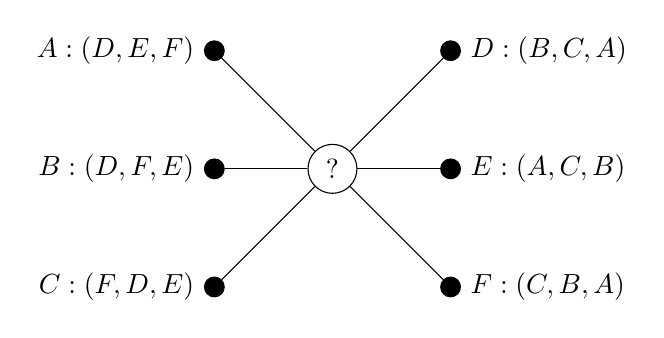
\begin{tikzpicture}[scale=0.5]

    % Suitors
    \node[draw, shape=circle, fill, inner sep=0, minimum size=0.25cm,
    label=left: {\(A: (D, E, F)\)}] (A) at (0, 0) {};
    \node[draw, shape=circle, fill, inner sep=0, minimum size=0.25cm, 
    label=left: {\(B: (D, F, E)\)}] (B) at (0, -3) {}; 
    \node[draw, shape=circle, fill, inner sep=0, minimum size=0.25cm, 
    label=left: {\(C: (F, D, E)\)}] (C) at (0, -6) {};

    % Reviewers
    \node[draw, shape=circle, fill, inner sep=0, minimum size=0.25cm, 
    label=right: {\(D: (B, C, A)\)}] (D) at (6, 0) {};
    \node[draw, shape=circle, fill, inner sep=0, minimum size=0.25cm, 
    label=right: {\(E: (A, C, B)\)}] (E) at (6, -3) {};
    \node[draw, shape=circle, fill, inner sep=0, minimum size=0.25cm,
    label=right: {\(F: (C, B, A)\)}] (F) at (6, -6) {};

    % Question mark node
    \node[draw, shape=circle] (q) at (3, -3) {?};
        
    % Lines into (?)
    \foreach \x in {A, B, C, D, E, F}
        \draw (\x) -- (q);

\end{tikzpicture}
\caption{A simple matching game represented on a bipartite
    graph.}\label{fig:matching_bipartite}

    \end{figure}

    Suppose we have the matching shown in Figure~\ref{fig:unstable_matching} for
    our game. This matching, \(M\) is valid since it is a bijection between 
    \(S\) and \(R\) but it is not stable. For instance, we have \((B, D)\) as a
    blocking pair since \(B\) would rather be matched with \(D\) than its 
    current match \(E\), and \(D\) would prefer to be matched with \(B\) than
    its current match \(A\).

    \begin{figure}[h]
        \centering
        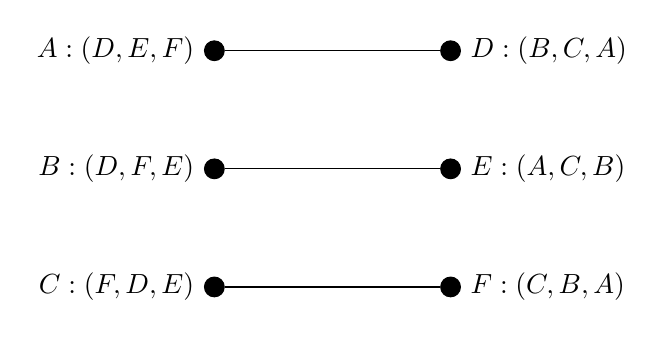
\begin{tikzpicture}[scale=0.5]

    % Suitors
    \node[draw, shape=circle, fill, inner sep=0, minimum size=0.25cm, 
    label=left: {\(A: (D, E, F)\)}] (A) at (0, 0) {};
    \node[draw, shape=circle, fill, inner sep=0, minimum size=0.25cm, 
    label=left: {\(B: (D, F, E)\)}] (B) at (0, -3) {}; 
    \node[draw, shape=circle, fill, inner sep=0, minimum size=0.25cm, 
    label=left: {\(C: (F, D, E)\)}] (C) at (0, -6) {};

    % Reviewers
    \node[draw, shape=circle, fill, inner sep=0, minimum size=0.25cm, 
    label=right: {\(D: (B, C, A)\)}] (D) at (6, 0) {};
    \node[draw, shape=circle, fill, inner sep=0, minimum size=0.25cm, 
    label=right: {\(E: (A, C, B)\)}] (E) at (6, -3) {};
    \node[draw, shape=circle, fill, inner sep=0, minimum size=0.25cm,
    label=right: {\(F: (C, B, A)\)}] (F) at (6, -6) {};

    % Lines
    \draw (A) -- (D);
    \draw (B) -- (E);
    \draw (C) -- (F);

\end{tikzpicture}
\caption{A example of an unstable matching for our
    game.}\label{fig:unstable_matching}

    \end{figure}

    We can make this matching stable by switching these pairs as in
    Figure~\ref{fig:stable_matching}. Here we have that each suitor is matched 
    with their most preferred reviewer so as not to form a blocking pair. We 
    call such a matching \emph{suitor-optimal}.

    \begin{figure}[h]
        \centering
        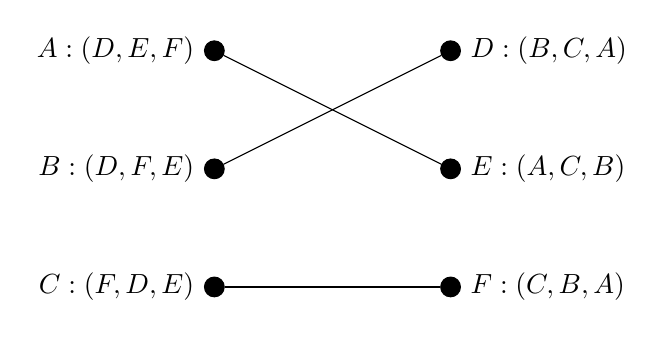
\begin{tikzpicture}[scale=0.5]

    % Suitors
    \node[draw, shape=circle, fill, inner sep=0, minimum size=0.25cm, 
    label=left: {\(A: (D, E, F)\)}] (A) at (0, 0) {};
    \node[draw, shape=circle, fill, inner sep=0, minimum size=0.25cm, 
    label=left: {\(B: (D, F, E)\)}] (B) at (0, -3) {}; 
    \node[draw, shape=circle, fill, inner sep=0, minimum size=0.25cm, 
    label=left: {\(C: (F, D, E)\)}] (C) at (0, -6) {};

    % Reviewers
    \node[draw, shape=circle, fill, inner sep=0, minimum size=0.25cm, 
    label=right: {\(D: (B, C, A)\)}] (D) at (6, 0) {};
    \node[draw, shape=circle, fill, inner sep=0, minimum size=0.25cm, 
    label=right: {\(E: (A, C, B)\)}] (E) at (6, -3) {};
    \node[draw, shape=circle, fill, inner sep=0, minimum size=0.25cm,
    label=right: {\(F: (C, B, A)\)}] (F) at (6, -6) {};

    % Lines
    \draw (A) -- (E);
    \draw (B) -- (D);
    \draw (C) -- (F);

\end{tikzpicture}
\caption{An example of a stable matching for our
    game.}\label{fig:stable_matching}

    \end{figure}
\end{example}


\balg%
    \caption{The hospital-resident algorithm
        (resident-optimal)}\label{alg:hospital_resident}
    \KwIn{a set of residents \(R\), a set of hospitals \(H\), a set of hospital
        capacities \(C\), two preference list functions \(f, g\)}
    \KwOut{a stable, resident-optimal mapping \(M\) between \(R\) and \(H\)}

    \For{\(h \in H\)}{%
        \(M^{-1}(h) \gets \emptyset\)
    }
    \While{There exists any unmatched \(r \in R\) with a non-empty preference
        list}{%
        Take any such resident \(r\) and their most preferred hospital \(h\)\;
        \(\textsc{MatchPair}(s, h)\)\;

        \If{\(\abs*{M^{-1}(h)} > c_h\)}{%
            Find their worst match \(r' \in M^{-1}(h)\)\;
            \(\textsc{UnmatchPair}(r', h)\)\;
        }
        \If{\(\abs*{M^{-1}(h)} = c_h\)}{%
            Find their worst match \(r' \in M^{-1}(h)\)\;
            \For{each successor \(s \in g(h)\) to \(r'\)}{%
                \(\textsc{DeletePair}(s, h)\)
            }
        }
    }
\ealg%

\balg%
    \caption{\textsc{MatchPair}}\label{alg:match}
    \KwIn{a resident \(r\), a hospital \(h\), a matching \(M\)}
    \KwOut{an updated matching \(M\)}

    \(M^{-1}(h) \gets M^{-1}(h) \cup \left\{r\right\}\)\;
\ealg%

\balg%
    \caption{\textsc{UnmatchPair}}\label{alg:unmatch}
    \KwIn{a resident \(r\), a hospital \(h\), a matching \(M\)}
    \KwOut{an updated matching \(M\)}

    \(M^{-1}(h) \gets M^{-1}(h) \setminus \left\{r\right\}\)\;
\ealg%

\balg%
    \caption{\textsc{DeletePair}}\label{alg:delete}
    \KwIn{a resident \(r\), a hospital \(h\)}
    \KwOut{updated preference lists}

    \(f(r) \gets f(r) \setminus \left\{h\right\}\)\;
    \(g(h) \gets g(h) \setminus \left\{r\right\}\)\;
\ealg%

\begin{algorithm}[H]
\caption{The proposed initialisation method}
    \begin{algorithmic}[0]
        \State{\textbf{Input:} a dataset \textbf{X}, with attribute sets \(A_1,
        \ldots, A_m\), and a number of modes to find \(k\)}
        \State{\textbf{Output:} a set of \(k\) initial modes \(\bar{\mu}\)\\}
        \\
        \Comment{Initialisation step}
        \State{\(\tilde{\mu} \gets \emptyset\)}
        \State{\(\bar{\mu} \gets \emptyset\)}
        \State{\(R \gets \emptyset\)}
        \State{\(S \gets \emptyset\)}
        \State{\(C \gets \{c_1, \ldots, c_k\}\)}

        \For{\(j = 1, \ldots, m\)}
            \For{\(s = 1, \ldots, d_j\)}
                \State{Calculate the relative frequency of each attribute value:
                    \(\frac{n(a_s^{(j)})}{N}\).}
	        \EndFor%
        \EndFor%
        \\
        \\
        \Comment{Find the set of virtual modes, \(\tilde{\mu}\), according to
        Huang's method.}
        \For{\(l = 1, \ldots, k\)}
            \For{\(j = 1, \ldots, m\)}
                \State{Consider the probability distribution given by:
                \(
                    \mathbb{P}(A_j) := \left(\frac{n(a_s^{(j)})}{N} : a_s^{(j)}
                    \in A_j\right)
                \)}
                \State{Sample \(a_{s^*}^{(j)}\) from \(A_j\) with respect to
                \(\mathbb{P}(A_j)\).}
                \State{\(\mu_j^{(l)} \gets a_{s^*}^{(j)}\)}
	        \EndFor%
            \State{\(\tilde{\mu} \gets \tilde{\mu} \cup
            \left\{\mu^{(l)}\right\}\)}
	    \EndFor%
        \\
        \\
        \Comment{Construct and solve a capacitated matching game.}
        \State{\(R \gets \tilde{\mu}\)}
        \For{\(r \in R\)}
            \State{\(c_r \gets 1\)}
            \State{Find the set of \(k\) vectors, \(S_r\), in \textbf{X} that 
            are the least dissimilar to \(r\).}
            \State{Arrange \(S_r\) into descending order of similarity.}
            \State{\(S \gets S \cup S_r\)}
        \EndFor%
        \For{\(r \in R\)}
            \State{\(g(r) \gets S_r\)}
        \EndFor%
        \State{Select a method for suitor preference lists and construct
        \(f(s)\) accordingly for each \(s \in S\).}
        \State{Solve the capacitated matching game defined by \((S, R, C)\) to
        obtain a matching \(M:~R~\to~S\).}
        \For{\(r \in R\)}
            \State{\(\bar{\mu} \gets \bar{\mu} \cup \{M(r)\}\)}
        \EndFor%
    \end{algorithmic}
\end{algorithm}


\section{Experimental results}\label{sec:results}

To give comparative results on the quality of the initialisation processes
considered in this work, four well-known, categorical, labelled datasets ---
breast cancer, mushroom, nursery, and soybean (large) --- will be clustered by
the \(k\)-modes algorithm with each of the initialisation processes. These
datasets have been chosen to fall in line with the established literature, and
for their relative sizes and complexities. Each dataset is openly available
under the UCI Machine Learning Repository~\cite{Dua2019}, and their
characteristics are summarised in Table~\ref{tab:dataset_summary}.

\begin{table}[htbp]
    \resizebox{\textwidth}{!}{%
        \begin{tabular}{lrrrlrr}
\toprule
{} &  No. rows &  No. cols &  No. classes &  Missing values &  Adjusted no. rows &  Adjusted no. classes \\
\midrule
Breast cancer &       699 &        10 &            2 &            True &                683 &                     2 \\
Mushroom      &      8124 &        22 &            2 &            True &               5644 &                     2 \\
Soybean       &       307 &        35 &           19 &            True &                266 &                    15 \\
Nursery       &     12960 &         8 &            5 &           False &              12960 &                     5 \\
\bottomrule
\end{tabular}

    }\caption{A summary of the benchmark datasets.}\label{tab:dataset_summary}
\end{table}

Clustering algorithms are often evaluated based on their performance as a
classifier~\cite{%
    Arthur2007,Cao2009,Cao2012,Huang1998,Ng2007,Olaode2014,Schaeffer2007%
}. This is a fundamentally flawed approach --- especially given that
classification belongs to an entirely different branch of learning. Moreover,
doing so requires a number of assumptions about the topology of the data within
the metric space that is being considered~\cite{Memoli2011}. One such assumption
is that the classes recorded in the data are indeed separable objects like
clusters.

This analysis does not consider evaluative metrics related to classification
such as accuracy, recall or precision. Instead, only internal measures are
considered such as the cost function defined in~\eqref{eq:cost}. This metric is
label-invariant and its values are comparable across the different
initialisation methods. Furthermore, the effect of each initialisation method
on the initial and final clusterings can be captured with the cost function. An
additional, and often useful, metric is the silhouette coefficient. This
measures the ratio between the intra-cluster cohesion and inter-cluster
separation of a particular clustering. Therefore, it could be used in a similar
way to reveal the effect of each initialisation method at the beginning and end
of a run of \(k\)-modes. Unfortunately, this metric loses its intuition under
the distance measure employed here and is omitted. The remaining performance
measures used are the number of iterations for the \(k\)-modes algorithm to
terminate and the time taken to terminate in seconds.

The final piece of information required in this analysis is a choice for \(k\)
for each dataset. An immediate choice is the number of classes that are present
in a dataset but, as stated above, this is not necessarily a fair or wise choice
since the classes may not be representative of true clusters. A popular strategy
for choosing an optimal number of clusters is known as the `elbow' method. The
aim of this method is to identify a kink (elbow) in a plot of number of clusters
against cost for a dataset. This kink suggests that an increase in \(k\) from
there would not sufficiently improve the performance of the model. On its own,
this method is vague and somewhat unreliable which raises a number of questions:
\begin{itemize}
    \item What constitutes a kink?
    \item How does one discern between multiple kinks?
    \item Is the decision subjective with respect to the observer?
\end{itemize}

Alas, an alternative `elbow' may be identified objectively by using
the knee point detection algorithm~\cite{Satopaa2011} where the maximal
value of \(k\) is taken to be \(\lfloor\sqrt{N}\rfloor\). This algorithm
identifies the value of \(k\) with the maximum curvature in the plot described
above by computation rather than inspection --- eliminating the concerns raised.
An example plot for the nursery dataset is given in
Figure~\ref{fig:nursery_costs} where the clustering is performed using Cao's
method.

\begin{figure}
    \centering
    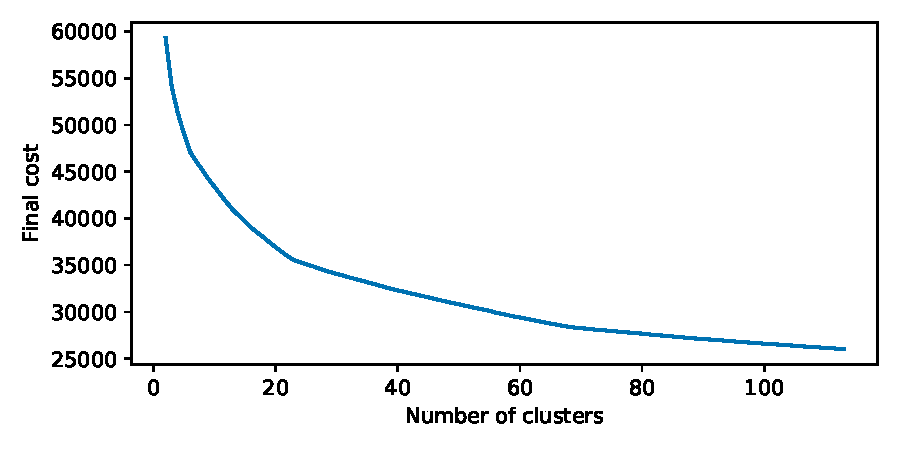
\includegraphics[width=.6\linewidth]{./img/elbow/nursery_costs.pdf}
    \caption{An elbow plot for the nursery dataset using Cao's initialisation
             method.}\label{fig:nursery_costs}
\end{figure}

\subsection{Elbow method}
\graphicspath{{./img/elbow/}}

Tables~\ref{tab:breast_cancer_summary_elbow}---\ref{tab:soybean_summary_elbow}
summarise the results of each initialisation method on the benchmark datasets
where the number of clusters has been determined by the knee point detection
algorithm. Each column shows the mean value of each metric and its standard
deviation in parentheses over 250
independent
repetitions of the \(k\)-modes algorithm.

\begin{table}
    \centering
    \resizebox{\textwidth}{!}{%
        \begin{tabular}{lllll}
\toprule
{} &      Initial cost &        Final cost & No. iterations &          Time \\
\midrule
Cao      &   2178.00 (0.000) &   1955.00 (0.000) &   4.00 (0.000) &  0.37 (0.025) \\
Huang    &  2123.12 (92.805) &  2023.80 (49.390) &   2.58 (0.810) &  0.25 (0.054) \\
Matching &  2110.68 (87.670) &  2015.42 (40.354) &   2.72 (0.834) &  0.21 (0.034) \\
\bottomrule
\end{tabular}

    }
    \captionof{table}{Summative metric results for the breast cancer dataset
    with \(k=8\).}\label{tab:breast_cancer_summary_elbow}\vspace{20pt}

    \resizebox{\textwidth}{!}{%
        \begin{tabular}{lllll}
\toprule
{} &         Initial cost &           Final cost & No. iterations &          Time \\
\midrule
Cao      &     29922.00 (0.000) &     29621.00 (0.000) &   2.00 (0.000) &  1.78 (0.066) \\
Huang    &  35112.67 (3286.612) &  31312.27 (1387.005) &   2.98 (1.012) &  2.74 (0.758) \\
Matching &  35237.67 (3201.877) &  31183.28 (1143.908) &   2.99 (0.924) &  1.79 (0.421) \\
\bottomrule
\end{tabular}

    }
    \captionof{table}{Summative metric results for the mushroom dataset with
    \(k=17\).}\label{tab:mushroom_summary_elbow}\vspace{20pt}

    \resizebox{\textwidth}{!}{%
        \begin{tabular}{lllll}
\toprule
{} &        Initial cost &          Final cost & No. iterations &          Time \\
\midrule
Cao      &    35544.00 (0.000) &    35544.00 (0.000) &   1.00 (0.000) &  4.98 (0.152) \\
Huang    &  37535.06 (372.596) &  37535.06 (372.596) &   1.00 (0.000) &  3.58 (0.121) \\
Matching &  37484.29 (327.467) &  37484.29 (327.467) &   1.00 (0.000) &  3.14 (0.141) \\
\bottomrule
\end{tabular}

    }
    \captionof{table}{Summative metric results for the nursery dataset with
    \(k=23\).}\label{tab:nursery_summary_elbow}\vspace{20pt}

    \resizebox{\textwidth}{!}{%
        \begin{tabular}{lllll}
\toprule
{} &       Initial cost &        Final cost & No. iterations &          Time \\
\midrule
Cao      &    1822.00 (0.000) &   1700.00 (0.000) &   4.00 (0.000) &  0.24 (0.009) \\
Huang    &  1964.56 (107.504) &  1832.92 (61.820) &   3.36 (0.875) &  0.23 (0.043) \\
Matching &   1929.50 (85.928) &  1829.54 (68.632) &   3.44 (1.110) &  0.15 (0.027) \\
\bottomrule
\end{tabular}

    }
    \captionof{table}{Summative metric results for the soybean dataset with
    \(k=8\).}\label{tab:soybean_summary_elbow}
\end{table}

\begin{figure}
    \begin{minipage}{.5\textwidth}
        \includegraphics[width=\linewidth]%
            {breast_cancer_cost_scatterplot.pdf}
    \end{minipage}
    \begin{minipage}{.5\textwidth}
        \includegraphics[width=\linewidth]%
            {breast_cancer_initial_cost_cdfplot.pdf}

        \includegraphics[width=\linewidth]%
            {breast_cancer_final_cost_cdfplot.pdf}
    \end{minipage}
\end{figure}

\begin{figure}
    \begin{minipage}{.5\textwidth}
        \includegraphics[width=\linewidth]%
            {mushroom_cost_scatterplot.pdf}
    \end{minipage}
    \begin{minipage}{.5\textwidth}
        \includegraphics[width=\linewidth]%
            {mushroom_initial_cost_cdfplot.pdf}

        \includegraphics[width=\linewidth]%
            {mushroom_final_cost_cdfplot.pdf}
    \end{minipage}
\end{figure}

\begin{figure}
    \begin{minipage}{.5\textwidth}
        \includegraphics[width=\linewidth]%
            {soybean_cost_scatterplot.pdf}
    \end{minipage}
    \begin{minipage}{.5\textwidth}
        \includegraphics[width=\linewidth]%
            {soybean_initial_cost_cdfplot.pdf}

        \includegraphics[width=\linewidth]%
            {soybean_final_cost_cdfplot.pdf}
    \end{minipage}
\end{figure}

\begin{figure}
    \begin{minipage}{.5\textwidth}
        \includegraphics[width=\linewidth]%
            {nursery_cost_scatterplot.pdf}
    \end{minipage}
    \begin{minipage}{.5\textwidth}
        \includegraphics[width=\linewidth]%
            {nursery_initial_cost_cdfplot.pdf}

        \includegraphics[width=\linewidth]%
            {nursery_final_cost_cdfplot.pdf}
    \end{minipage}
\end{figure}


\subsection{Number of classes}
\graphicspath{{./img/nclasses/}}

\begin{table}
    \centering
    \resizebox{\textwidth}{!}{%
        \begin{tabular}{lllll}
\toprule
{} &       Initial cost &         Final cost & No. iterations &          Time \\
\midrule
Cao      &    3315.00 (0.000) &    3172.00 (0.000) &   2.00 (0.000) &  0.13 (0.005) \\
Huang    &  3393.80 (120.772) &  3348.51 (144.849) &   1.54 (0.653) &  0.10 (0.024) \\
Matching &  3406.73 (111.686) &  3355.56 (144.621) &   1.61 (0.638) &  0.09 (0.018) \\
\bottomrule
\end{tabular}

    }
    \captionof{table}{Summative metric results for the breast cancer dataset
    with \(k=8\).}\label{tab:breast_cancer_summary_nclasses}\vspace{20pt}

    \resizebox{\textwidth}{!}{%
        \begin{tabular}{lllll}
\toprule
{} &         Initial cost &           Final cost & No. iterations &          Time \\
\midrule
Cao      &     37662.00 (0.000) &     37662.00 (0.000) &   1.00 (0.000) &  1.10 (0.142) \\
Huang    &  41720.20 (2519.647) &  38612.64 (2086.246) &   3.14 (1.471) &  2.04 (0.759) \\
Matching &  42297.98 (2265.532) &  39496.56 (2681.581) &   3.36 (1.439) &  1.62 (0.567) \\
\bottomrule
\end{tabular}

    }
    \captionof{table}{Summative metric results for the mushroom dataset with
    \(k=17\).}\label{tab:mushroom_summary_nclasses}\vspace{20pt}

    \resizebox{\textwidth}{!}{%
        \begin{tabular}{lllll}
\toprule
{} &        Initial cost &          Final cost & No. iterations &          Time \\
\midrule
Cao      &    35544.00 (0.000) &    35544.00 (0.000) &   1.00 (0.000) &  4.98 (0.152) \\
Huang    &  37535.06 (372.596) &  37535.06 (372.596) &   1.00 (0.000) &  3.58 (0.121) \\
Matching &  37484.29 (327.467) &  37484.29 (327.467) &   1.00 (0.000) &  3.14 (0.141) \\
\bottomrule
\end{tabular}

    }
    \captionof{table}{Summative metric results for the nursery dataset with
    \(k=23\).}\label{tab:nursery_summary_nclasses}\vspace{20pt}

    \resizebox{\textwidth}{!}{%
        \begin{tabular}{lllll}
\toprule
{} &       Initial cost &        Final cost & No. iterations &          Time \\
\midrule
Cao      &    1822.00 (0.000) &   1700.00 (0.000) &   4.00 (0.000) &  0.24 (0.009) \\
Huang    &  1964.56 (107.504) &  1832.92 (61.820) &   3.36 (0.875) &  0.23 (0.043) \\
Matching &   1929.50 (85.928) &  1829.54 (68.632) &   3.44 (1.110) &  0.15 (0.027) \\
\bottomrule
\end{tabular}

    }
    \captionof{table}{Summative metric results for the soybean dataset with
    \(k=8\).}\label{tab:soybean_summary_nclasses}
\end{table}

\begin{figure}
    \begin{minipage}{.5\textwidth}
        \includegraphics[width=\linewidth]%
            {breast_cancer_cost_scatterplot.pdf}
    \end{minipage}
    \begin{minipage}{.5\textwidth}
        \includegraphics[width=\linewidth]%
            {breast_cancer_initial_cost_cdfplot.pdf}

        \includegraphics[width=\linewidth]%
            {breast_cancer_final_cost_cdfplot.pdf}
    \end{minipage}
\end{figure}

\begin{figure}
    \begin{minipage}{.5\textwidth}
        \includegraphics[width=\linewidth]%
            {mushroom_cost_scatterplot.pdf}
    \end{minipage}
    \begin{minipage}{.5\textwidth}
        \includegraphics[width=\linewidth]%
            {mushroom_initial_cost_cdfplot.pdf}

        \includegraphics[width=\linewidth]%
            {mushroom_final_cost_cdfplot.pdf}
    \end{minipage}
\end{figure}

\begin{figure}
    \begin{minipage}{.5\textwidth}
        \includegraphics[width=\linewidth]%
            {soybean_cost_scatterplot.pdf}
    \end{minipage}
    \begin{minipage}{.5\textwidth}
        \includegraphics[width=\linewidth]%
            {soybean_initial_cost_cdfplot.pdf}

        \includegraphics[width=\linewidth]%
            {soybean_final_cost_cdfplot.pdf}
    \end{minipage}
\end{figure}

\begin{figure}
    \begin{minipage}{.5\textwidth}
        \includegraphics[width=\linewidth]%
            {nursery_cost_scatterplot.pdf}
    \end{minipage}
    \begin{minipage}{.5\textwidth}
        \includegraphics[width=\linewidth]%
            {nursery_initial_cost_cdfplot.pdf}

        \includegraphics[width=\linewidth]%
            {nursery_final_cost_cdfplot.pdf}
    \end{minipage}
\end{figure}


\section{Conclusion}\label{sec:conclusion}

In this paper a novel initialisation method for the \(k\)-modes was introduced
that built on the method set out in the seminal paper~\cite{Huang1998}. The new
method models the final `replacement' process in the original as an instance of
the Hospital-Resident Assignment Problem that may be solved to be mathematically
fair and stable.

Following a thorough description of the \(k\)-modes algorithm and the
established initialisation methods, a comparative analysis was conducted amongst
the three initialisations using both benchmark and artificial datasets. This
analysis revealed that the proposed initialisation was able to outperform both
of the other methods when the choice of \(k\) was optimised according to a
mathematically rigorous elbow method. However, the proposed method was unable to
beat Cao's method (established in~\cite{Cao2009}) when an external framework was
imposed on each dataset by choosing \(k\) to be the number of classes present.

The proposed method should be employed over Cao's when there are no hard
restrictions on what \(k\) may be, or if there is no immediate evidence that the
dataset at hand has some notion of high density. Otherwise, Cao's method remains
the most reliable initialisation in terms of computational time and final cost.


\clearpage%
\bibliography{references}
\clearpage%
\appendix\section{Appendix}

\subsection{Proof that simple matching dissimilarity is a metric}

Let \(\mathcal A\) be a categorical attribute space and let the dissimilarity
function, \(d : \mathcal A^2 \to \mathbb R\), be defined as
in~\eqref{eq:dissim}. Then \(d\) is a metric such that for all \(x, y, z \in
\mathcal A\):
\begin{multicols}{2}
    \begin{enumerate}[label=(\roman*)]
        \item \(d\left(x, y\right) \geq 0\)
        \item \(d\left(x, y\right) = 0 \iff x = y\)
        \item \(d\left(x, y\right) = d\left(y, x\right)\)
        \item \(d\left(x, y\right) + d\left(y, z\right) \geq
            d\left(x, z\right)\)
    \end{enumerate}
\end{multicols}

\begin{proof}
    Consider any \(x,y,z \in \mathcal A\).
    \begin{enumerate}[label=(\roman*)]
        \item If \(x = y\), then \(x_j = y_j\) for all \(j = 1, \ldots, m\).
            Then it immediately follows that \(d(x,y) = 0\). Otherwise,
            \(\delta\left(x_j, y_j\right) = 1\) for at least one
            \(j = 1, \ldots, m\). Therefore, \(d(x, y) \geq 1\), as required.
        \item Consider any \(x, y \in \mathcal A\) such that \(d(x, y) = 0\).
            Then \(d(x, y) = 0 \iff \delta\left(x_j, y_j\right) = 0\) for all
            \(j = 1, \ldots, m \iff x_j = y_j\) for all
            \(j = 1, \ldots, m \iff x = y\), as required.
        \item This follows from the definition
            of \(\delta\) in~\eqref{eq:dissim}
        \item Without ambiguity, let \(x, y, z\) each be represented as a set of
            its elements. Then an alternative form for \(d\) may be considered
            where \(d(x, y) = m - \abs*{x \cap y}\). With this, it is sufficient
            to show:
            \[
                \left(m - \abs*{x \cap y}\right)
                + \left(m - \abs*{y \cap z}\right)
                \geq m - \abs*{x \cap z}
            \]
            That is,
            \(\abs*{x \cap y} - \abs*{x \cap z} + \abs*{y \cap z} \leq m\). So,
            \[
                \begin{aligned}
                    \abs*{x \cap y} - \abs*{x \cap z} + \abs*{y \cap z}
                    & \leq
                    \abs*{x \cap \left(y \setminus z\right)} + \abs*{y \cap z}\\
                    & \leq
                    \abs*{y \setminus z} + \abs*{y \cap z}\\
                    & = \abs*{y} = m
                \end{aligned}
            \]
    \end{enumerate}

    Therefore, \(d\) satisfies conditions (i) \-- (iv) and is a metric.
\end{proof}


\end{document}
